\documentclass[border=10pt]{standalone}
\usepackage[svgnames]{xcolor}
\usepackage{amsmath}
\usepackage{pgfplots}
\pgfplotsset{compat=newest}
\usepackage[sfdefault]{FiraSans}
\usepackage{FiraMono}
\renewcommand*\familydefault{\sfdefault}
\begin{document}
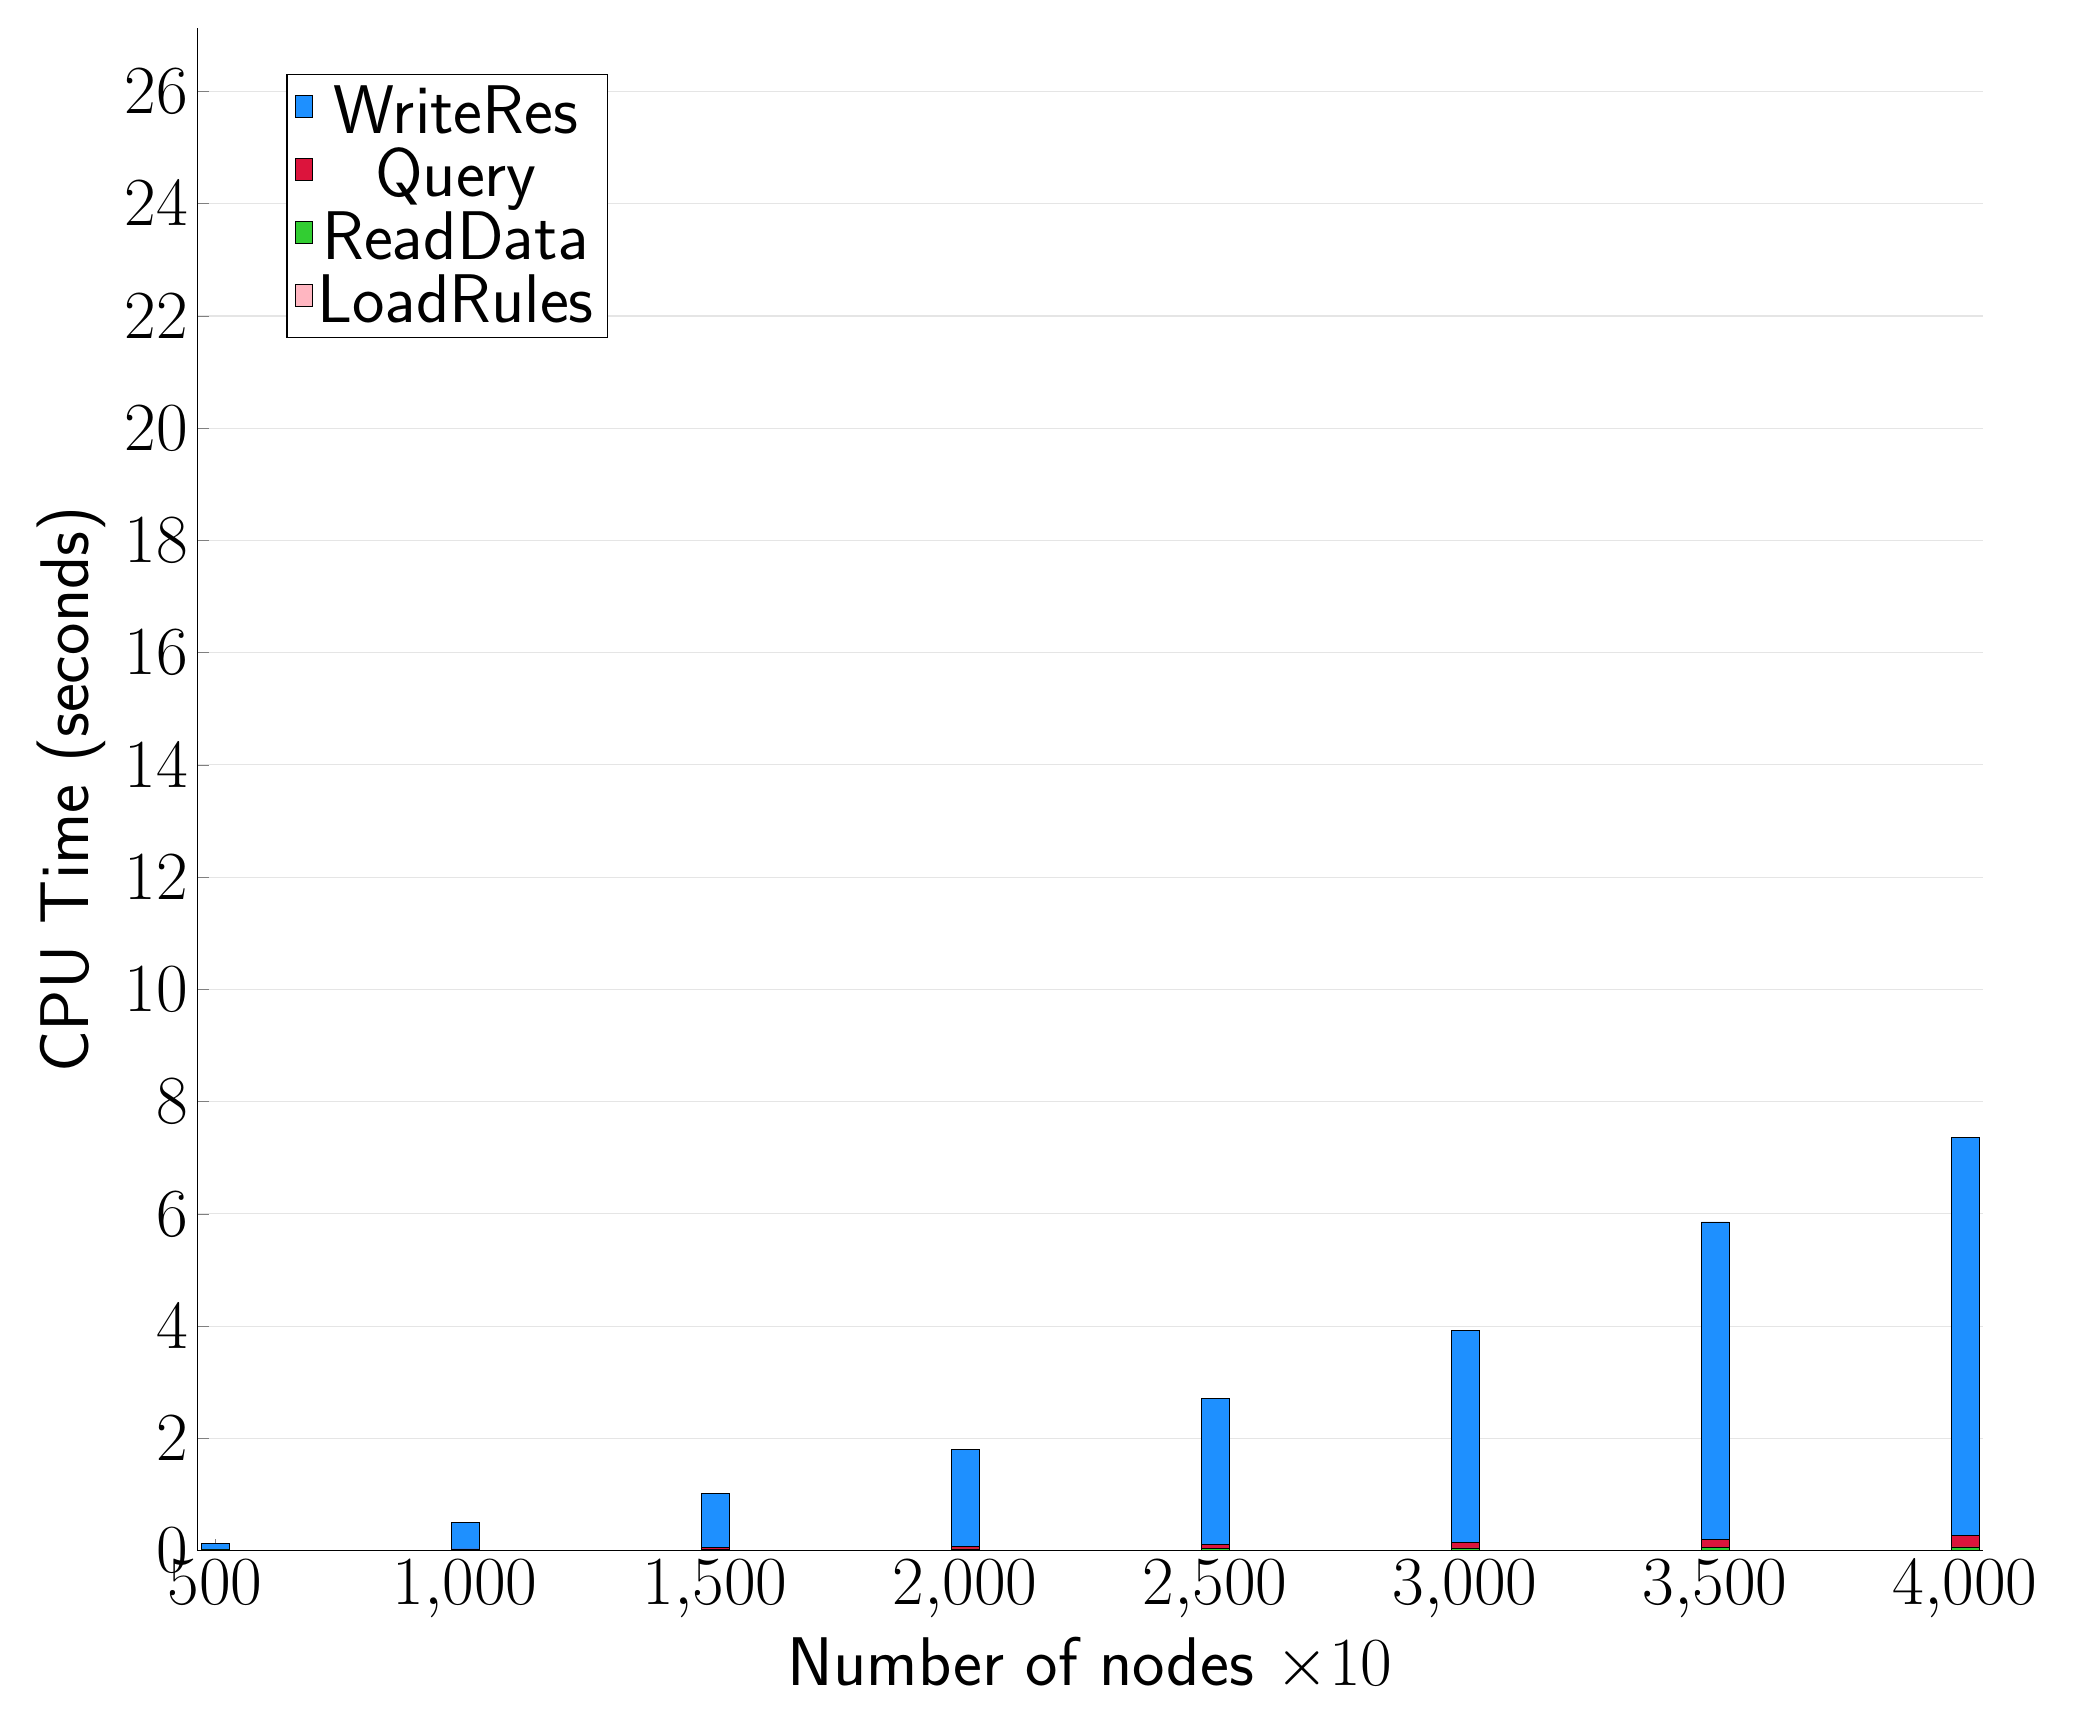
\begin{tikzpicture}
\begin{axis}[
   ybar stacked,
   width=2\textwidth,
   bar width=0.35cm,
   ymajorgrids, tick align=inside,
   major grid style={draw=gray!20},
   xtick=data,
   ymin=0, ymax=27.127176920572918,
   axis x line*=bottom,
   axis y line*=left,
   enlarge x limits=0.01,
   legend style={
       at={(0.23, 0.97)},
       anchor=north east,
       legend columns=1,
       font=\Huge,
   },
   ylabel={CPU Time (seconds)},
   xlabel={Number of nodes $\times 10$},
   label style={font=\Huge},
   tick label style={font=\Huge},
]
\addlegendimage{fill=DodgerBlue, draw=black, line width=0.2pt}
\addlegendentry{WriteRes}
\addlegendimage{fill=Crimson, draw=black, line width=0.2pt}
\addlegendentry{Query}
\addlegendimage{fill=LimeGreen, draw=black, line width=0.2pt}
\addlegendentry{ReadData}
\addlegendimage{fill=LightPink, draw=black, line width=0.2pt}
\addlegendentry{LoadRules}
\addplot +[fill=LightPink, draw=black, line width=0.2pt] coordinates {
(500, 0.0043983333333333366)
(1000, 0.0036113333333333344)
(1500, 0.0035723333333333336)
(2000, 0.003583)
(2500, 0.00308)
(3000, 0.004263333333333337)
(3500, 0.0046926666666666636)
(4000, 0.004095666666666667)
};
\addplot +[fill=LimeGreen, draw=black, line width=0.2pt] coordinates {
(500, 0.00975666666666667)
(1000, 0.014732333333333333)
(1500, 0.024073)
(2000, 0.028184999999999998)
(2500, 0.033819999999999996)
(3000, 0.04633166666666667)
(3500, 0.055771666666666664)
(4000, 0.061406666666666665)
};
\addplot +[fill=Crimson, draw=black, line width=0.2pt] coordinates {
(500, 0.0029769999999999966)
(1000, 0.014081999999999999)
(1500, 0.028643000000000002)
(2000, 0.04636833333333334)
(2500, 0.069826)
(3000, 0.10206466666666668)
(3500, 0.14394099999999999)
(4000, 0.21151266666666668)
};
\addplot +[fill=DodgerBlue, draw=black, line width=0.2pt] coordinates {
(500, 0.11326433333333334)
(1000, 0.4781503333333334)
(1500, 0.9658199999999999)
(2000, 1.730109)
(2500, 2.611098666666667)
(3000, 3.767497)
(3500, 5.653893)
(4000, 7.086441666666666)
};
\end{axis}
\end{tikzpicture}

\end{document}
